%%%%%%%%%%%%%%%%%%%%%%%%%%%%%%%%%%%%%%%%%
% Beamer Presentation
% LaTeX Template
% Version 1.0 (10/11/12)
%
% This template has been downloaded from:
% http://www.LaTeXTemplates.com
%
% License:
% CC BY-NC-SA 3.0 (http://creativecommons.org/licenses/by-nc-sa/3.0/)
%
%%%%%%%%%%%%%%%%%%%%%%%%%%%%%%%%%%%%%%%%%

%----------------------------------------------------------------------------------------
%	PACKAGES AND THEMES
%----------------------------------------------------------------------------------------

\documentclass[10pt]{beamer}

\mode<presentation> {

% The Beamer class comes with a number of default slide themes
% which change the colors and layouts of slides. Below this is a list
% of all the themes, uncomment each in turn to see what they look like.

%\usetheme{default}
%\usetheme{AnnArbor}
%\usetheme{Antibes}
%\usetheme{Bergen}
%\usetheme{Berkeley}
%\usetheme{Berlin}
%\usetheme{Boadilla}
%\usetheme{CambridgeUS}
%\usetheme{Copenhagen}
%\usetheme{Darmstadt}
%\usetheme{Dresden}
%\usetheme{Frankfurt}
%\usetheme{Goettingen}
%\usetheme{Hannover}
%\usetheme{Ilmenau}
%\usetheme{JuanLesPins}
%\usetheme{Luebeck}
\usetheme{Madrid}
%\usetheme{Malmoe}
%\usetheme{Marburg}
%\usetheme{Montpellier}
%\usetheme{PaloAlto}
%\usetheme{Pittsburgh}
%\usetheme{Rochester}
%\usetheme{Singapore}
%\usetheme{Szeged}
%\usetheme{Warsaw}

% As well as themes, the Beamer class has a number of color themes
% for any slide theme. Uncomment each of these in turn to see how it
% changes the colors of your current slide theme.

%\usecolortheme{albatross}
%\usecolortheme{beaver}
%\usecolortheme{beetle}
%\usecolortheme{crane}
%\usecolortheme{dolphin}
%\usecolortheme{dove}
%\usecolortheme{fly}
%\usecolortheme{lily}
%\usecolortheme{orchid}
%\usecolortheme{rose}
%\usecolortheme{seagull}
%\usecolortheme{seahorse}
%\usecolortheme{whale}
%\usecolortheme{wolverine}

%\setbeamertemplate{footline} % To remove the footer line in all slides uncomment this line
%\setbeamertemplate{footline}[page number] % To replace the footer line in all slides with a simple slide count uncomment this line

%\setbeamertemplate{navigation symbols}{} % To remove the navigation symbols from the bottom of all slides uncomment this line
}

\usepackage{graphicx} % Allows including images
\usepackage{booktabs} % Allows the use of \toprule, \midrule and \bottomrule in tables
\usepackage[utf8]{inputenc}
\usepackage[T2A]{fontenc}
\usepackage[russian]{babel}
\usepackage{ragged2e} 
\usepackage{amsmath}
\usepackage{hyperref}
%----------------------------------------------------------------------------------------
%	TITLE PAGE
%----------------------------------------------------------------------------------------

\title[]{Исправление грамматических ошибок в домене низкоресурсных языков } % The short title appears at the bottom of every slide, the full title is only on the title page

\author{Хабутдинов Ильдар Айратовивч} % Your name
\institute[МФТИ] % Your institution as it will appear on the bottom of every slide, may be shorthand to save space
{
Научный руководитель: к.ф.-м.н. А. В. Грабовой \\
Московский Физико-Технический Институт \\ % Your institution for the title page
\medskip
\textit{} % Your email address
}
\date{\today} % Date, can be changed to a custom date

\begin{document}

\begin{frame}
\titlepage % Print the title page as the first slide
\end{frame}

\begin{frame}
\frametitle{Задача исправления грамматических ошибок } % Table of contents slide, comment this block out to remove it
\justifying
{\color{blue}{Проблема}} \\
Интерпретируемое автоматическое исправление текстовых последовательностей. \\
% {\color{blue}{Задача}} \\
% Предложить метод инъективного отображения из множества произвольных символьных последовательностей в множество наперед заданных целевых последовательностей. \\
~\\
{\color{blue}{Задача}} \\
Исправление грамматических ошибок в домене низкоресурсных языков. \\
~\\
{\color{blue}{Метод решения}} \\
Метод инъективного отображения из множества произвольных символьных последовательностей в множество наперед заданных целевых последовательностей. 
~\\
Предложенный метод решения задачи основан на сведении задачи нахождения последовательности корректирующих преобразований к задаче поиска оптимального редакционного предписания  между исходной и целевой последовательностями.



\end{frame}

%----------------------------------------------------------------------------------------
%	PRESENTATION SLIDES
%----------------------------------------------------------------------------------------

\begin{frame}
\frametitle{Визуализация постановки задачи}


\begin{figure}[h]
    \centering
    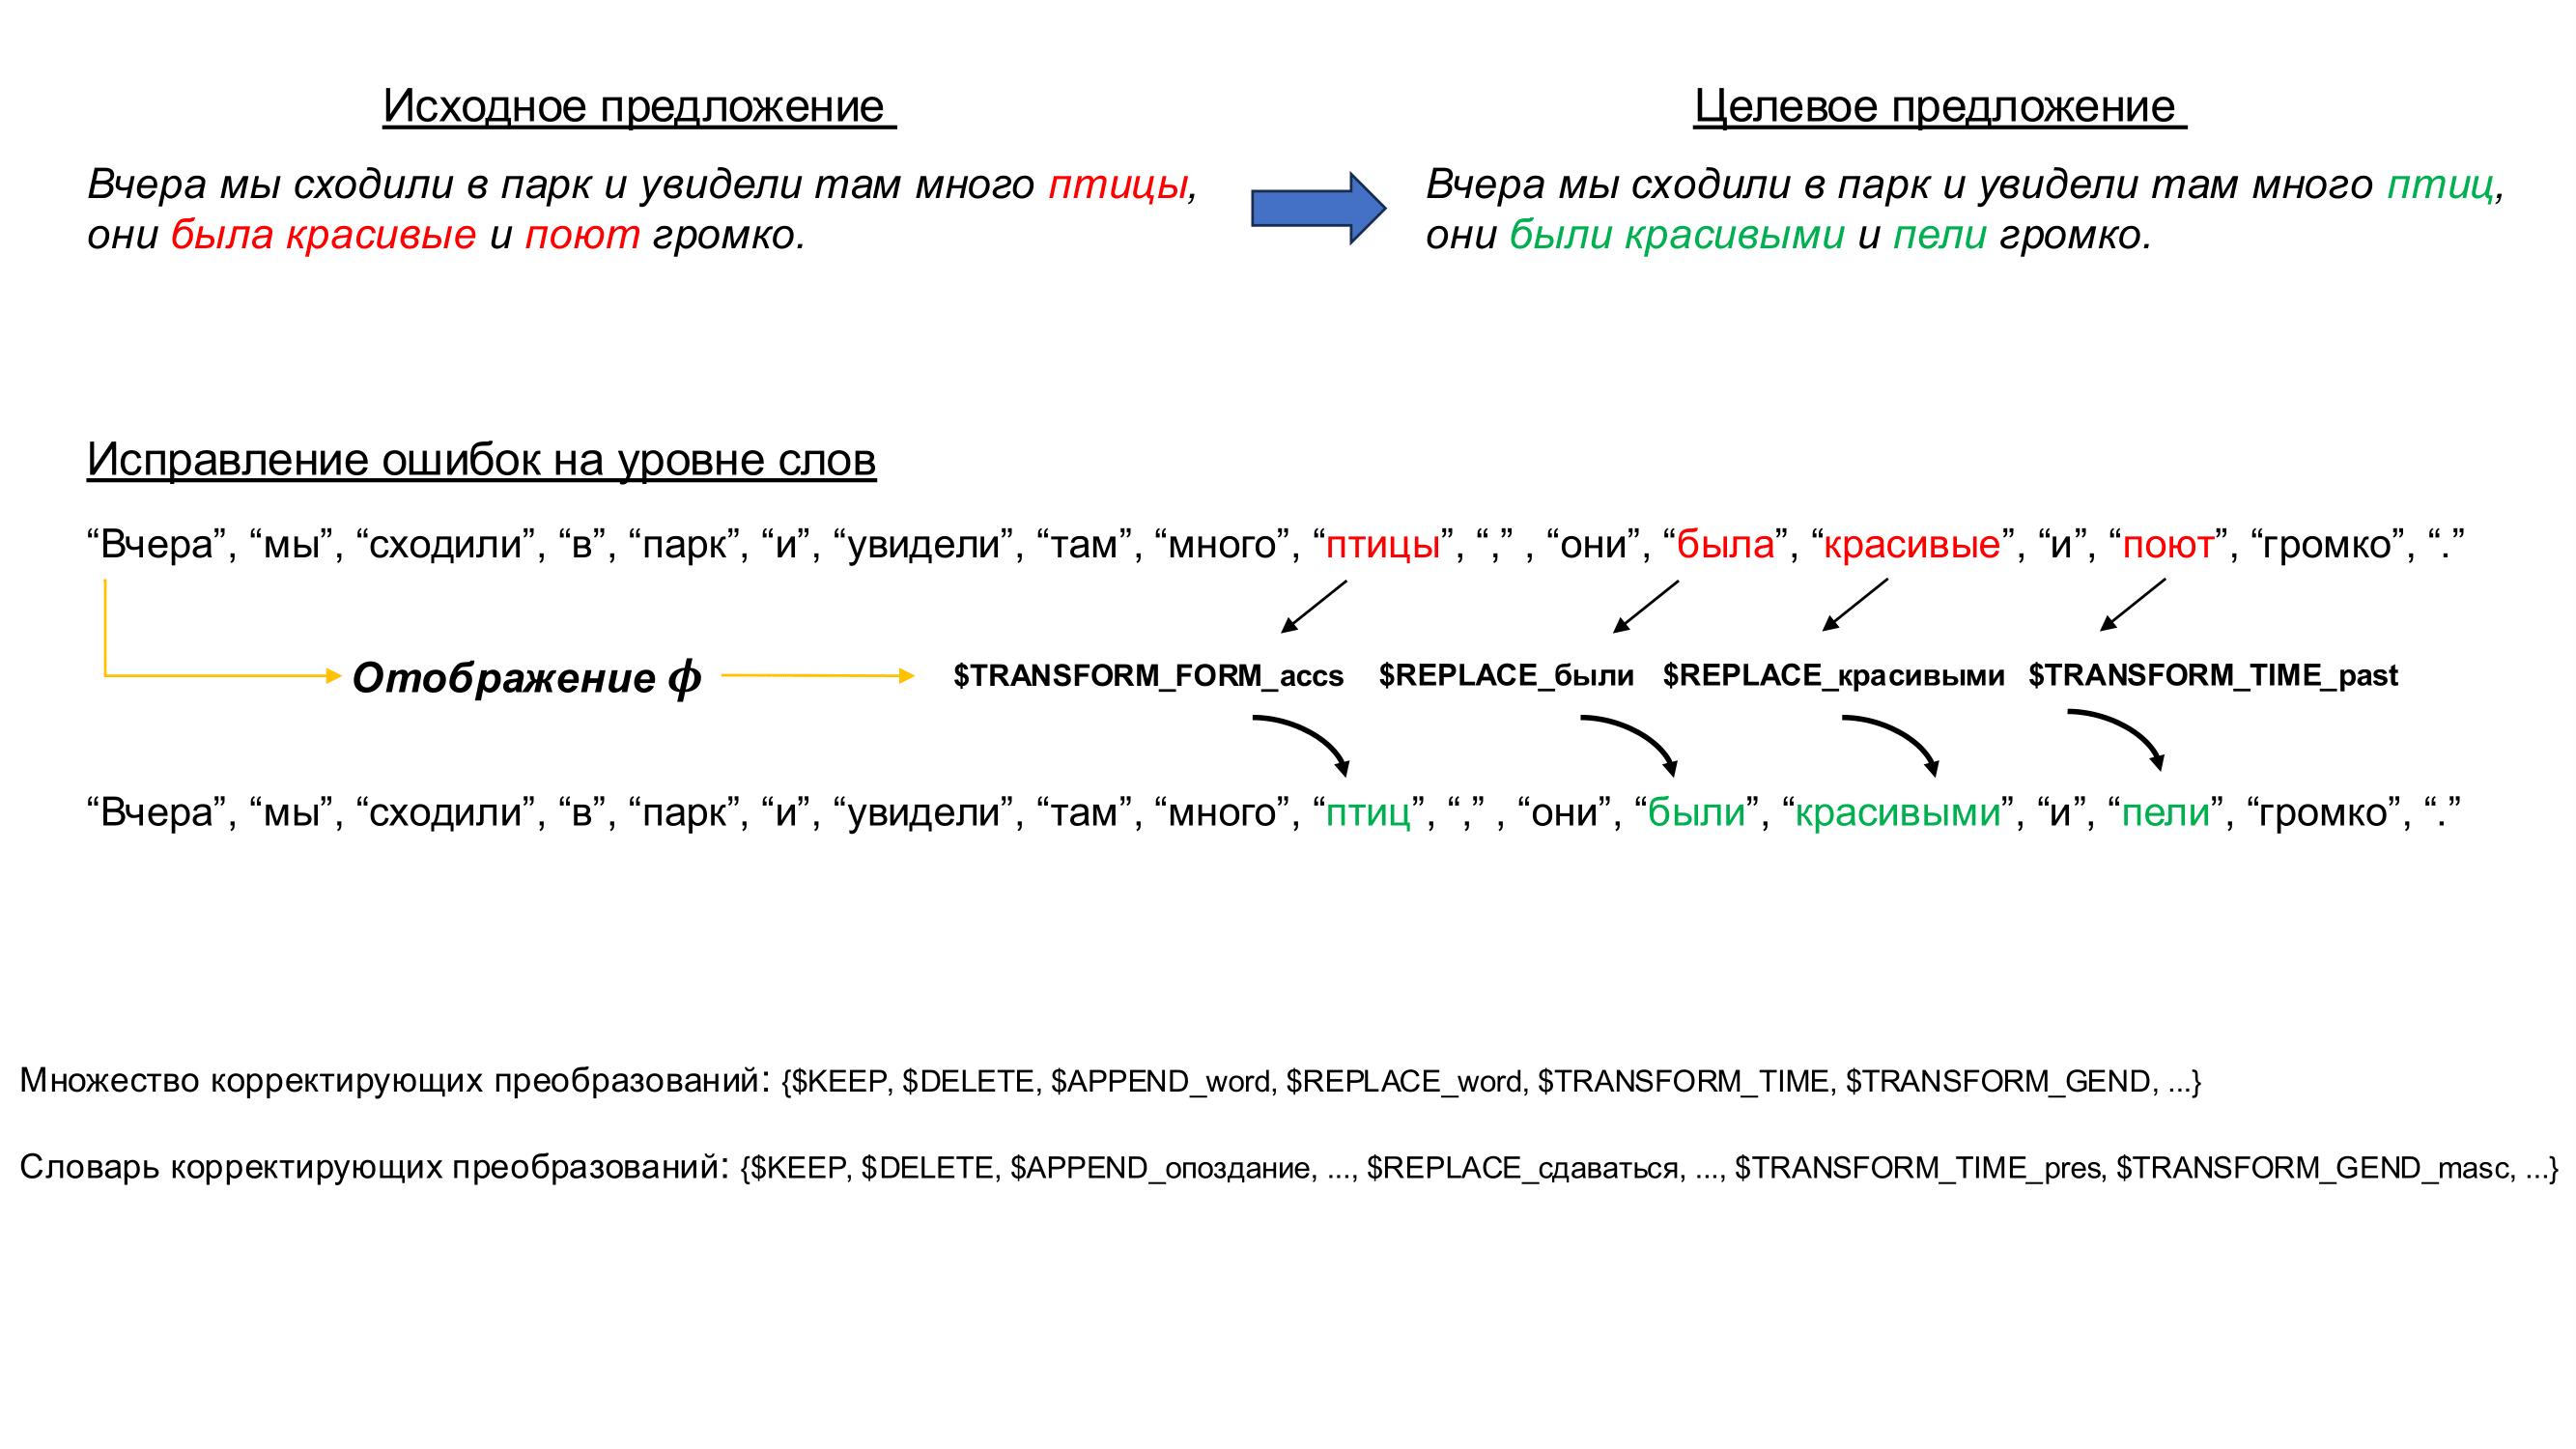
\includegraphics[width=1.0\textwidth]{picture-1.png} % Укажите имя файла
    % \label{fig:pdf_as_image}
\end{figure}


\end{frame}


\begin{frame}
\frametitle{Задача построения корректирующих преобразований}
%алфавит, токенизатор, множество слов, создан множество коррект преобразов, экспертные знания
\justifying
\begin{small}
Заданы: 
\begin{itemize}
\item Алфавит \( \Sigma \) 
\item Язык \( \Sigma^* \): множество всех возможных строк над \(\Sigma\), включая пустую строку \(\varepsilon\) 
\item Словарь токенов: \( V \subseteq \Sigma^* \)
\end{itemize}
Задан токенизатор $ T: s \to \{x_1, x_2, ..., x_n\}, s \in \Sigma^*, x_j \in V$ \\
 Множество символьных послед. с разбиением на послед. токенов длины $n_i$, \[ \mathcal{X} = \{s_i | s_i=\{x_1, x_2, ... , x_{n_i}\} | x_j \in V, 1 \le j \le n_i\}_{i = 0}^N, \] \\
Множество целевых последовательностей с разбиением длины m_i:
\\\[\mathcal{Y} = \{t_i | t_i =\{y_1, y_2, ... , y_{m_i}\} | y_j \in V, 1 \le j \le m_i\}_{i = 0}^N \] \\

Множество корректирующих преобразований \( \mathcal{F} \), \(f \in \mathcal{F}: V \to V \)

На основе заданного множества необходимо построить словарь $ K $ корректирующих преобразований размера p  \[ K = \{f_i: a_i \to b_i | f_i \in \mathcal{F}, a_i, b_i \in V\}_{i = 0}^{p} \]

%W словарь слов, словарь корректирующих преобразований, функция которая выдает множество коррект преобр 

Требуется найти отображение $\phi : \{x_1, x_2, ..., x_{n_i}\} \to  \{f_1, f_2, ..., f_{n_i}\}$ 
\[ \{f_1, f_2, ..., f_{n_i}\}: \{f_1, f_2, ..., f_{n_i}\} \circ \{x_1, x_2, ..., x_{n_i}\} \rightarrow \{y_1, y_2, ..., y_{m_i}\}, где k_j \in K \]

Символом $\circ$ обозначено применение корр. преобразования $f_j$ к токену $x_j$.

\end{small}
\end{frame}


\begin{frame}
\frametitle{Корректирующие преобразования для русского языка}

\justifying
\begin{small}

\begin{itemize}
\item Алфавит \( {\Sigma}_{\text{ru}} \) — это множество из 33 букв русского алфавита: $\Sigma_{\text{ru}} = \{ \text{А, Б, В, ..., Э, Ю, Я} \}$
\item Язык \( \Sigma^*_{\text{ru}} \): множество всех возможных строк над \(\Sigma\), включая пустую строку \(\varepsilon\) 
\item В качестве словаря токенов взят словарь русских слов \( V_{\text{ru}} \subseteq \Sigma^*_{\text{ru}} \)
\item Задан токенизатор для русского языка $T_{\text{ru}}$
\end{itemize}


Строится словарь корректирующих преобразований $ K $\footnote{\href{https://link.springer.com/article/10.1134/S0361768824700129}{\textbf{Khabutdinov, I.A., Chashchin, A.V., Grabovoy, A.V. et al.} RuGECToR: Rule-Based Neural Network Model for Russian Language Grammatical Error Correction. }}, который состоит из элементов:
\begin{enumerate}
\item Преобразования APPEND и REPLACE с использованием 2500 самых частых русских слов на основе коэффициента Жуайна;
\item Преобразования DELETE и KEEP для удаления слова и cохранения слова соответственно;
\item преобразования, общие для всех слов: слияние и разделение слов, изменение регистра букв и т.д.;
\item специальные преобразования для изменения соответствующих частей речи: изменение падежа, рода, лица, времени, числа;
\item преобразования для исправления распространенных ошибок в глаголах: ться/тся и при/пре.
\end{enumerate}



% Соответственно данным корректирующим преобразованиям был сгенерирован синтетический набор данных.

% \begin{table}[]
% \begin{tabular}{|l|l|l|l|}
%   \hline
%   Источник данных & \#предложений & \%ошибок в предложениях  \\ \hline
%   Wiki + Essays & $10\,000\,000$ & $\approx 100\%$  \\ \hline
%   Proza + Essays & $1\,000\,000$ & $\approx 50\%$ \\ \hline
% \end{tabular}
% \end{table}

\end{small}

\end{frame}

\begin{frame}
\frametitle{Автоматическое построение корректирующих преобразований}
%обобщенные корректирующие преобразования для любого алфавита
%кванторами описать независимость от алфавита и тд.

Проблемы ручной разработки корректирующих преобразований при переходе к произвольному языку:

\begin{itemize}
\item Необходимо определение множества корректирующих преобразований
\item необходимо составление словаря корректирующих преобразований;
\item необходимо осуществить лингвистический анализ грамматических правил данного языка;
% \item необходимо аннотирование данных согласно разработанным корректирующим преобразованиям: для синтетических данных требуется создание алгоритма выравнивания и алгоритма генерации ошибок, для реальных данных требуется разметка ассесоров.
\end{itemize}
~\\
Решение: введение обобщенного множества корректирующих преобразований, переход к исправлению ошибок и разбиению символьных последовательностей на уровне подслов.

\end{frame}



% g-transformations perform task-specific opera- tions such as: change the case of the current token (CASE tags), merge the current token and the next token into a single one (MERGE tags) and split the current token into two new tokens (SPLIT tags). Moreover, tags from NOUN NUMBER and VERB FORM transformations encode grammatical prop- erties for tokens. For instance, these transforma- tions include conversion of singular nouns to plu- rals and vice versa or even change the form of reg- ular/irregular verbs to express a different number or tense.



%------------------------------------------------

\begin{frame}
\frametitle{Обобщенные корректирующие преобразования}

\justifying
\begin{small}
Заданы: 
\begin{itemize}
\item Произвольный алфавит \( \Sigma_{\text{any}} \) 
\item Произвольный язык \( \Sigma_{\text{any}}^* \): множество всех возможных строк над \(\Sigma_{\text{any}} \), включая пустую строку \(\varepsilon\) 
\item Словарь токенов: \( V_{\text{any}} \subseteq \Sigma_{\text{any}}^* \)
\item Токенизатор $T_{\text{any}}$
\end{itemize}
%переделать в свойство
\textbf{Условие достижимости.} Заданы произвольные конечные символьные последовательности $s$ и $t$. Токенизатор $ A $ удовлетворяет условию достижимости, если любую последовательность  $ A(t) $ можно получить из любой другой последовательности $ A(s) $ за конечное число операций вставки, удаления и замены. \\
~\\
%утв для WP токенизации выполняется

Если пара \((V_{\text{any}}, T_{\text{any}})\) удовлетворяет \textbf{условию достижимости}, то минимальное достаточное множество корректирующих преобразований $\mathcal{F}$ состоит из элементов:  

\begin{enumerate}
\item KEEP --- оставить токен без изменения
\item REPLACE\_t --- заменить токен $x_{j}$ произвольным токеном $t$
\item DELETE --- удалить токен $x_{j}$
\item APPEND\_t --- добавить токен $t$ после токена $x_{j}$
\end{enumerate}

\color{red}{Замечание: $T_{\text{ru}}$ не удовлетворяет условию достижимости}

\end{small}

\end{frame}


\begin{frame}
\frametitle{Определение редакционного предписания}
\justifying
\begin{small}

% \textbf{Доказательство.} Доказательство проведем от противного.

% Предположим, что существуют такие конечные строки \( s \) и \( t \), для которых последовательности токенов \( A(s) \) и \( A(t) \), порожденные WordPiece токенизатором:
% \[
% A(s) = [a_1, a_2, \ldots, a_n], \quad A(t) = [b_1, b_2, \ldots, b_m],
% \]
% \textbf{невозможно преобразовать друг в друга} с помощью корректирующих преобразований. Это предположение означает, что между последовательностями \( A(s) \) и \( A(t) \) существует фундаментальная разница, которую нельзя устранить указанными операциями.
% \begin{itemize}
% WordPiece токенизатор разбивает строку \( s \) на последовательность токенов \( A(s) \) на основе словаря и жадного алгоритма. 
% Для любой строки \( s \) разбиение \( A(s) \) единственно и полностью определяется содержимым строки и словарем.
% Пусть \( s \) и \( t \) — произвольные строки. Их последовательности токенов \( A(s) \) и \( A(t) \) являются конечными, так как строки имеют конечную длину.
% \end{itemize}

% Таким образом, любая из последовательностей состоит из конечного числа токенов, принадлежащих словарю.
% Невозможность применения преобразования $w_i$ к произвольному токену $t_i$ означает, что $t_i \notin WT \rightarrow $ противоречие.  

\textbf{Опр. Редакционное предписание --- это последовательность корретирующих преобразований, необходимых для получения целевой последовательности из исходной, имеющая минимальное количество операций вставки, замены и удаления.}
~\\
~\\
Пусть  $ D_{i,j} $ --- это расстояние редактирования между префиксами $s[0..i]$ и $t[0..j]$ длины i и j. Где $ D_{0, j} = 0 $ и $D_{i, 0} = 0$. Остальные значения определяются рекуррентным соотношением:

\begin{equation*}
    D_{i, j} = \begin{cases}
      D_{i-1, j-1}, s[i]=t[j] \\
      1 + min⁡\{D_{i-1,j}, D_{i, j-1}, D_{i-1, j-1}\}, else 
    \end{cases}
\end{equation*}

{\begin{figure}
    \captionsetup{}
	\subfloat{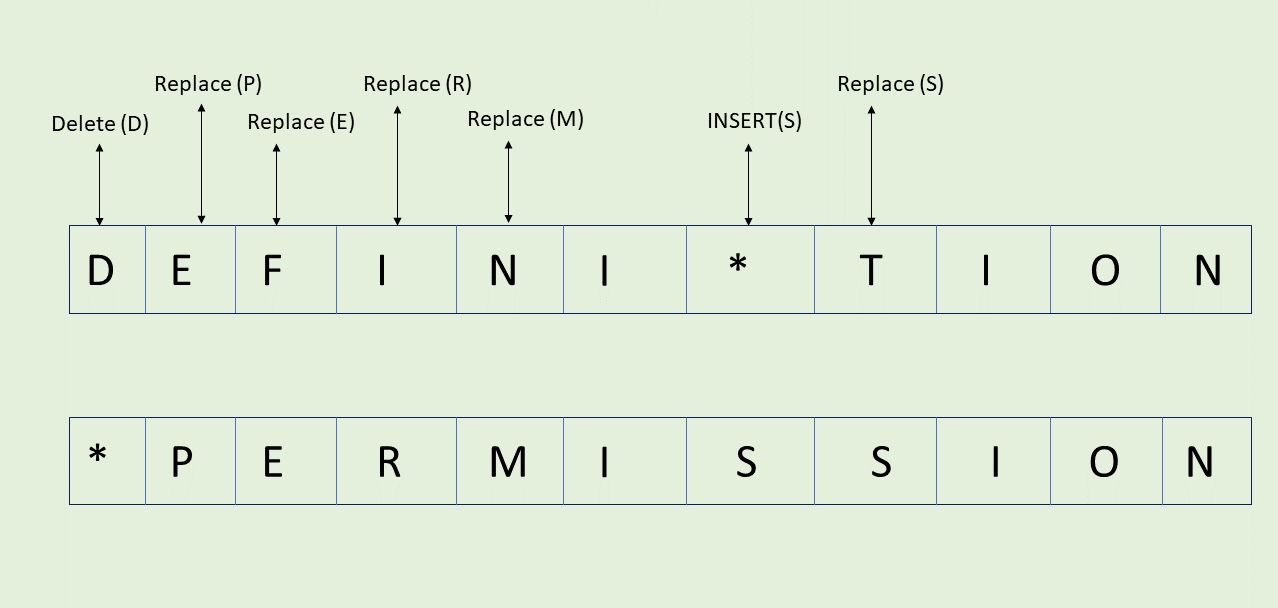
\includegraphics[width=0.6\textwidth]{EDIT_DISTANCE.jpg}}
\end{figure}}


\end{small}



\end{frame}

%------------------------------------------------

% \begin{frame}
% \frametitle{Последовательность корректирующих преобразований}

% \begin{small}    
% Пусть  $ D_{i,j} $ - это расстояние редактирования между префиксами $s[0..i]$ и $t[0..j]$ длины i и j. Где $ D_{0, j} = 0 $ и $D_{i, 0} = 0$. Остальные значения определяются рекуррентным соотношением:

% \begin{equation*}
%     D_{i, j} = \left \begin{cases}
%       D_{i-1, j-1}, s[i]=t[j] \\
%       1 + min⁡\{D_{i-1,j}, D_{i, j-1}, D_{i-1, j-1}\}, else 
%     \end{cases}\
% \end{equation*}

% Опр. Редакционное предписание - это последовательность корретирующих преобразований, необходимых для получения целевой последовательности из исходной, которая при этом содержит минимальное количество преобразований replace, append, delete.

% \textbf{Утв. Количество возможных редакционных предписаний равно количеству путей в графе подзадач, имеющих минимальную стоимость.}

% \textbf{Доказательство.} Давайте рассмотрим граф подзадач, где каждая вершина соответствует состоянию пары индексов \( (i,j) \), и ребра графа отражают возможные операции редактирования между последовательностями $s$ и $t$ длиной $n$ и $m$ соответственно:


% \begin{itemize}
% \item Если символы \( s[i] \) и \( t[j] \) равны, то можно перейти по диагонали без изменения (операция \textit{keep}).
% \item Если символы \( s[i] \) и \( t[j] \) различны, то возможны следующие операции:
%     \begin{itemize}
%     \textit{Замена} (replace): переход по диагонали \( (i-1, j-1) \),
%     \end{itemize}
% \end{itemize}

% \end{small}

% \end{frame}


\begin{frame}
\frametitle{Граф подзадач для редакционного предписания}

\begin{small}    

% \begin{itemize}
    % \begin{itemize}
    % \textit{Вставка} (append): переход из \( (i, j-1) \),
    % \textit{Удаление} (delete): переход из \( (i-1, j) \).
    % \end{itemize}
% \end{itemize}

% Редакционное предписание соответствует пути минимальной стоимости, проходящего от вершины \( (n, m) \) до вершины  \( (0, 0) \). Каждый путь имеет стоимость, равную количеству операций редактирования, где:
% \begin{itemize}
% Стоимость операции \textit{replace}, \textit{append} и \textit{delete} равна 1, а \textit{keep} равна 0
% \end{itemize}

% Так как стоимость изменяющих операций перехода одинакова, то может существовать несколько путей, которые приводят к минимальному значению $\rightarrow$ справедливость утверждения следует из определения редакционного предписания.

Граф подзадач, где каждая вершина --- пара индексов \( (i,j) \), ребра графа --- возможные корректирующие преобразования между последовательностями $s$ и $t$:


\begin{itemize}
\item Если $ s[i] = t[j], $ то переход по диагонали без изменений --- операция \textit{keep}.
\item Если символы \( s[i] \) и \( t[j] \) различны, то возможны следующие операции:\\
    \textit{Замена} (replace): переход по диагонали $ (i-1, j-1) $,\\
    \textit{Вставка} (append): переход из \( (i, j-1) \),\\
    \textit{Удаление} (delete): переход из \( (i-1, j) \).
\end{itemize}

\textbf{Утв. Количество возможных редакционных предписаний равно количеству путей в графе подзадач, имеющих минимальную стоимость.}

{\begin{figure}
    \captionsetup{}
	\subfloat{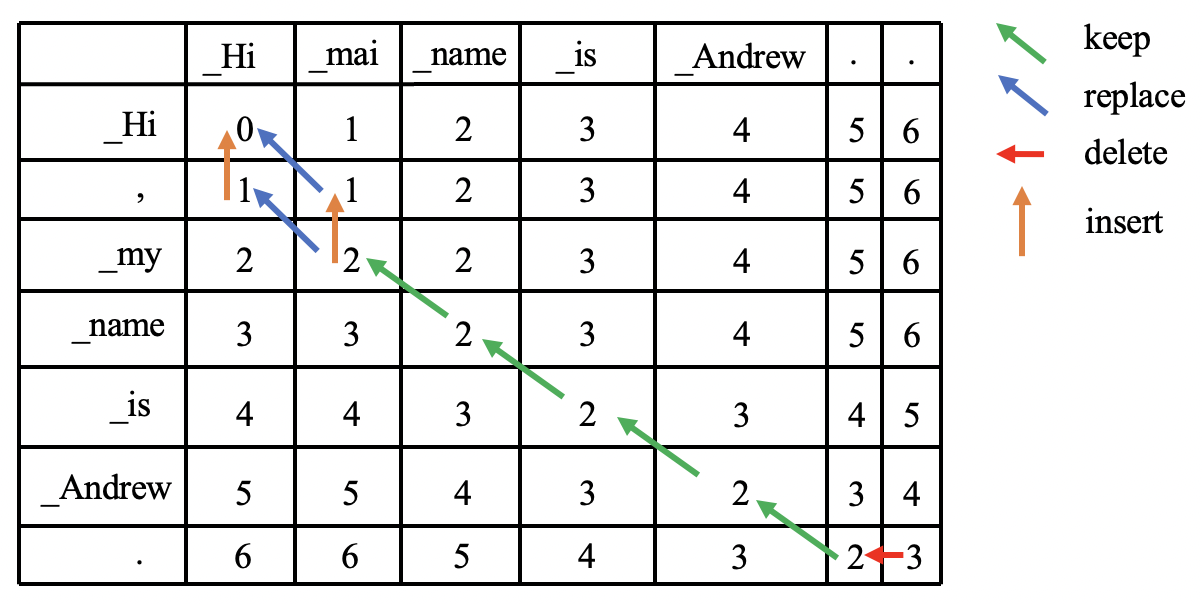
\includegraphics[width=0.45\textwidth]{backtracking.png}}
\end{figure}}

Редакционные предписания --- \{{\color{red} delete .} ; {\color{orange}insert \_my} ; {\color{blue}replace \_mai with ,}\} и \{{\color{red} delete .} ; {\color{orange}insert ,} ; {\color{blue}replace \_mai with \_my}\}

\end{small}

\end{frame}


% \begin{frame}
% \frametitle{Предложенный метод: поиск оптимального РП}

% \begin{small}    
% Обозначим $EP_k = \{e_{1}, e_{2}, ..., e_{o_k}\}  $ множетсво редакционных предписаний для пары последовательностей ($s_k$, $t_k$), где $o_k$ –– количество редакционных предписаний для $k$-й пары. 

% Для того чтобы найти оптимальное редакционное предписание для $k$-ой пары, мы учитываем сходство исходных и целевых токенов при применении правила replace. \\
% Пусть $R_l \subset e_l, l \in \{1, 2, ..., o_k\}$ - множество всех правил replace мощностью $p_l$ для произвольного редакционного предписания $ e_l$: 

% \begin{align*}
%     R_l =\{replace\_{t_1}_{i}\_{t_2}_{i}\}_{i=0}^{p_l}, 
% \end{align*}

% где исходный токенов ${t_1}_{i} \in s_k$, целевой токен ${t_2}_{i} \in t_k$. 

% Давайте введем сходство токенов:

% \begin{align*}
%     \sigma_l = \sum_{i=0}^{p_l}{LevenshteinDist({t_1}_{i}\_{t_2}_{i})}
% \end{align*}
% где $LevenshteinDist$ - функция, вычисляющая расстояние Левенштейна между $t_{1_i}$ и $t_{2_i}$ на уровне символов внутри токенов.


% \end{small}

% \end{frame}

\begin{frame}
\frametitle{Поиск оптимального редакционного предписания}
\justifying
\begin{small}    

Обозначим $EP_k = \{e_{1}, e_{2}, ..., e_{o_k}\}  $ множество редакционных предписаний для пары ($s_k$, $t_k$), где $o_k$ --- количество редакционных предписаний для $k$-й пары. 
~\\
~\\
Для нахождения оптимального редакционного предписания в $k$-ой паре, мы учитываем сходство исходных и целевых токенов для коррект. преобр. replace.
~\\
~\\
Пусть $R_l \subset e_l, l \in \{1, 2, ..., o_k\}$ - множество всех правил replace мощностью $p_l$ для произвольного редакционного предписания $ e_l$: 
\begin{align*}
    R_l =\{replace\_{t_1}_{i}\_{t_2}_{i}\}_{i=0}^{p_l}, 
\end{align*}

где исходный токенов ${t_1}_{i} \in s_k$, целевой токен ${t_2}_{i} \in t_k$. 
~\\
~\\
Введем сходство токенов как:
\begin{align*}
    \sigma_l = \sum_{i=0}^{p_l}{LevenshteinDist({t_1}_{i}\_{t_2}_{i})}
\end{align*}
где $LevenshteinDist$ - функция, вычисляющая расстояние Левенштейна между $t_{1_i}$ и $t_{2_i}$ на уровне символов внутри токенов. \\
~\\
\textbf{Утв. Редакционное предписание $e^*_{l}: l= argmin\{\sigma_1, \sigma_2, ..., \sigma_{o_k}\} $ является оптимальным.} \\
~\\

\end{small}

\end{frame}

\begin{frame}
\frametitle{Преимущества предложенного метода}
Преимущества данного подхода:

\begin{enumerate}
\item Данный метод предложен для целого класса токенизаторов, для которых выполнено условие достижимости;
\item нет необходимости в ручной разработке словаря грамматических правил, следовательно, может быть обобщено на любой низкоресурсный язык;
\item множество корректирующих преобразований не зависит от языка;
\item нет необходимости в ручной разработке словаря корректирующих правил $K$, корректирующие преобразования строятся путем нахождения редакционного предписания.
\end{enumerate}
\end{frame}

% \begin{frame}
% \frametitle{Архитектура модели}

% {\begin{figure}
%     \captionsetup{}
% 	\subfloat{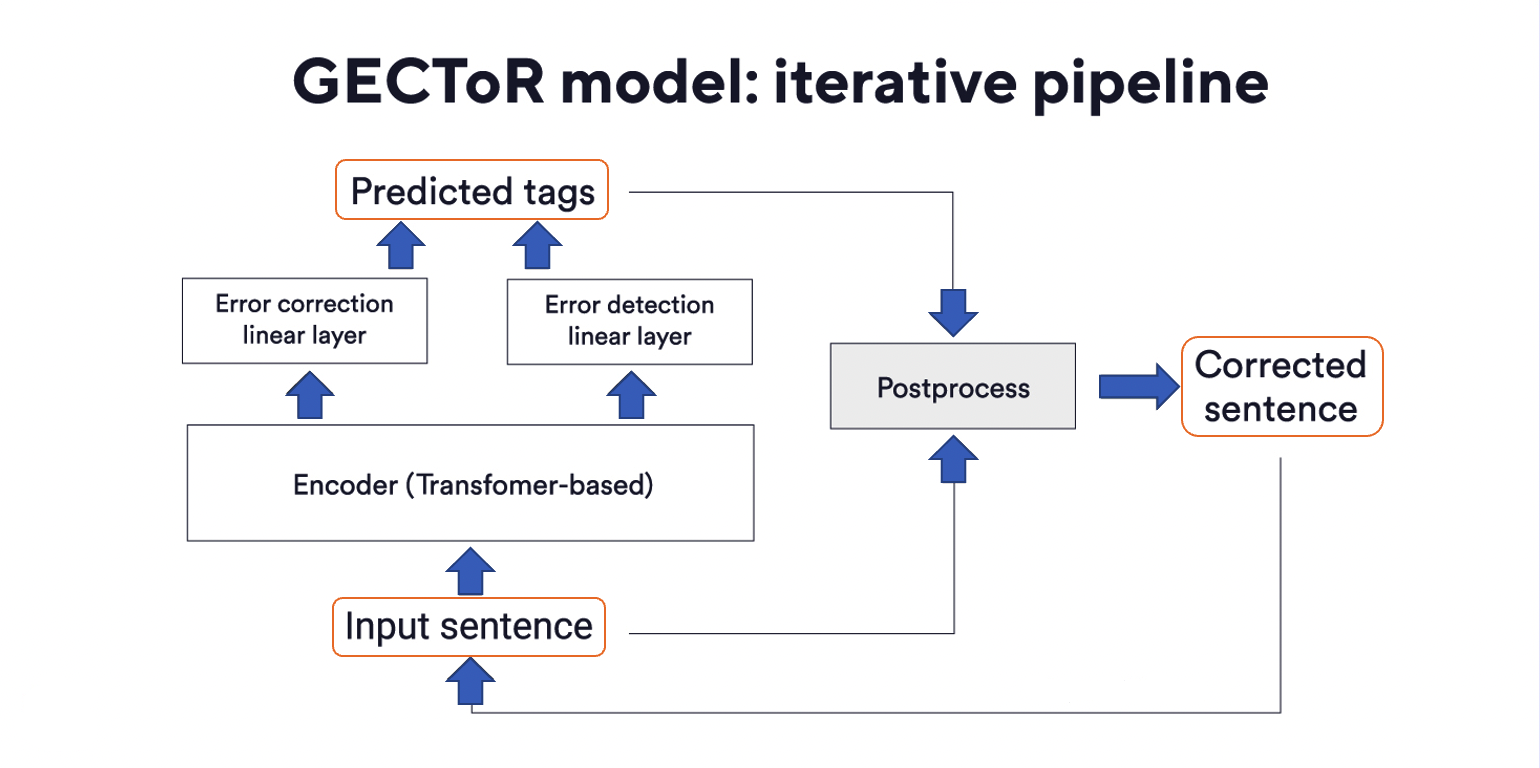
\includegraphics[width=1.0\textwidth]{GEC-scheme.png}}
% \end{figure}}
% \end{frame}

\begin{frame}
\frametitle{Эксперимент с корр. преобразованиями русского языка}
\begin{table}[ht!]
\begin{center}
\begin{tabular}{|l|l|l|l|l|}
  \hline
  Система & Этап обучения & $P$ & $R$ & $ F_{0.5} $\\ \hline
  RuGECToR & \RomanNumeralCaps{1} & 88.4 & \textbf{67.1} & \textbf{83.1} \\ \hline
  RuGECToR & \RomanNumeralCaps{2} & \textbf{88.5} & 65.1 & 82.5 \\ \hline
\end{tabular}
\end{center}
\caption{Оценка работы модели на синтетическом тестовом наборе данных}
\end{table}

\begin{table}[ht!]
\begin{center}
\begin{tabular}{|l|l|l|l|l|}
  \hline
  Система & Обучающие данные & $P$ & $R$ & $ F_{0.5} $\\ \hline
  Classifiers (learner) & RULEC & 22.6 & 4.8 & 12.9 \\ \hline
  Classifiers (min sup.) & RULEC & 38.0 & 7.5 & 21.0 \\ \hline
  MT & RULEC & 30.6 & 2.9 & 10.6 \\ \hline
  RuGECToR & Synthetic (\RomanNumeralCaps{1} stage) & 23.6 & 5.6 & 14.3 \\ \hline
  RuGECToR & Synthetic (\RomanNumeralCaps{2} stages) & \textbf{40.8} & \textbf{7.9} & \textbf{22.2} \\ \hline
\end{tabular}
\end{center}
\caption{Сравнение работы моделей на наборе данных RULEC}
\end{table}

Модель достигает $F_{0.5}$ = $22.2$. Этот результат выше бейзлайна, несмотря на то, что модель не обучалась на этом наборе данных.



\end{frame}


\begin{frame}
\frametitle{Эксперимент с обобщенными корр. преобразованиями}

% {\begin{figure}
%     \captionsetup{}
% 	\subfloat{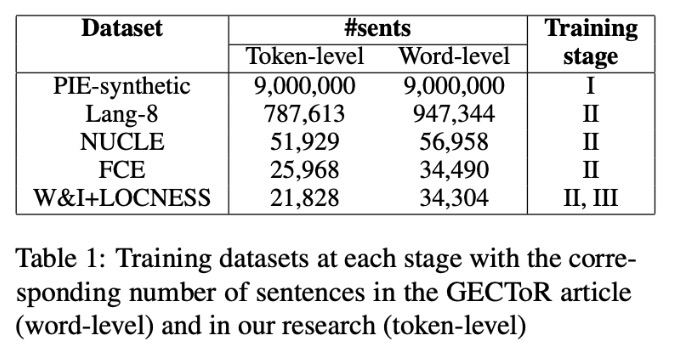
\includegraphics[width=0.5\textwidth]{data.jpg}}
% \end{figure}}
\begin{small}

\begin{table}
  \centering
  \small 
  \begin{tabular}{c*{2}{c}c}
    \hline
    \multirow{\textbf{\shortstack{Dataset}}} & \multicolumn{2}{c}{\textbf{\#sents}} & \multirow{\textbf{Training}}  \\
     & Subword-level  & Word-level & \textbf{stage}\\
    \hline
     PIE-synthetic &  9,000,000 & 9,000,000 & I \\
     Lang-8 & 787,613 & 947,344 & II  \\
     NUCLE & 51,929 & 56,958 & II  \\
     FCE & 25,968 & 34,490 & II \\
     W\&I+LOCNESS & 21,828 & 34,304 & II, III \\
    \hline
  \end{tabular}
 \caption{Обучающие наборы данных для каждого этапа с соответствующим количеством предложений для модели на уровне слов и модели на уровне подслов.}
  \label{tab:data}
\end{table}

% {\begin{figure}
%     \captionsetup{}
% 	\subfloat{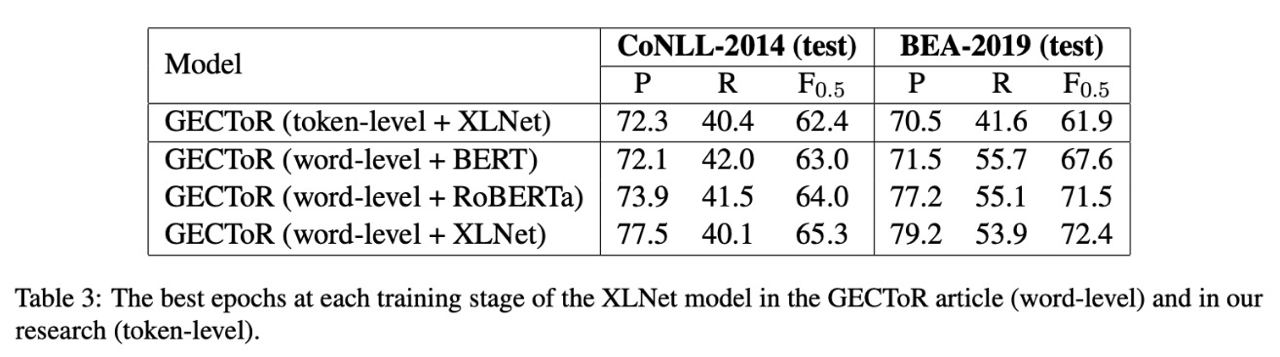
\includegraphics[width=0.7\textwidth]{comparison.jpg}}
% \end{figure}}

\begin{table}
  \centering
  \begin{tabular}{lcccccc}
    \hline
    \multirow{Model} & \multicolumn{3}{c}{\textbf{CoNLL-2014 (test)}} & \multicolumn{3}{c}{\textbf{BEA-2019 (test)}} \\
     & P & R & $F_{0.5}$ & P & R & ${F}_{0.5}$ \\
    \hline
    GECToR (subword-level + XLNet) & 72.3 & 40.4 & 62.4 & 70.5 & 41.6 & 61.9 \\
    \hline
    GECToR (word-level + BERT) & 72.1 & \textbf{42.0} & 63.0 & 71.5 & \textbf{55.7} & 67.6 \\ 
    GECToR (word-level + RoBERTa) & 73.9 & 41.5 & 64.0 & 77.2 & 55.1 & 71.5 \\
    GECToR (word-level + XLNet) & \textbf{77.5} & 40.1 & \textbf{65.3} & \textbf{79.2} & 53.9 & \textbf{72.4} \\
    % GECToR (word-level + BERT + RoBERTa + XLNet) & 78.2 & 41.5 & 66.5 & 78.9 & 58.2 & 73.6 \\
    \hline
  \end{tabular}
  \caption{Сравнение работы модели на уровне подслов с моделями на уровне слов.}
  \label{tab:result}
  
\end{table}

\end{small}

\end{frame}

\begin{frame}
\frametitle{Выносится на защиту}

\begin{itemize}
\item Предложено множество корректирующих преобразований для русского языка.
\item Модель RuGECToR, аппроксимирующая последовательность корректирующих преобразований.
\item Предложено множество обобщенных корректирующих преобразований.
\item Доказано, что для предложенного множества выполняется условие достижимости.
\item Модель GECToR, аппроксимирующая последовательность корректирующих преобразований на уровне подслов.
\end{itemize}


\end{frame}


\begin{frame}{Список работ автора по теме диссертации}
\justifying
{
\scriptsize
\textbf{Публикации}

\begin{enumerate}
\item \textbf{Khabutdinov, I.A., Chashchin, A.V., Grabovoy, A.V. et al.} RuGECToR: Rule-Based Neural Network Model for Russian Language Grammatical Error Correction. Program Comput Soft 50, 315–321 (2024). https://doi.org/10.1134/S0361768824700129 
\item \textbf{K. Varlamova, I. Khabutdinov and A. Grabovoy}, "Automatic Spelling Correction for Russian: Multiple Error Approach," 2023 Ivannikov Ispras Open Conference (ISPRAS), Moscow, Russian Federation, 2023, pp. 169-175, doi: 10.1109/ISPRAS60948.2023.10508161.
\item \textbf{Gritsai, German \& Khabutdinov, Ildar \& Grabovoy, Andrey}. (2024). Multi-head Span-based Detector for AI-generated Fragments in Scientific Papers. 220-225. 10.18653/v1/2024.sdp-1.21. 
\item \textbf{K. Grashchenkov, A. Grabovoy and I. Khabutdinov}, "A Method of Multilingual Summarization For Scientific Documents," 2022 Ivannikov Ispras Open Conference (ISPRAS), Moscow, Russian Federation, 2022, pp. 24-30, doi: 10.1109/ISPRAS57371.2022.10076852.
\item \textbf{Gritsai, German \& Voznyuk, Anastasia \& Khabutdinov, Ildar \& Grabovoy, Andrey.} (2024). Advacheck at GenAI Detection Task 1: AI Detection Powered by Domain-Aware Multi-Tasking. 10.48550/arXiv.2411.11736. 
\item \textbf{Khabutdinov, I.A., Krinitskiy, M.A. & Belikov, R.A.} Identifying Cetacean Mammals in High-Resolution Optical Imagery Using Anomaly Detection Approach Employing Machine Learning Models. Moscow Univ. Phys. 78 (Suppl 1), S149–S156 (2023). https://doi.org/10.3103/S0027134923070147
      
\end{enumerate}

\textbf{Выступления с докладом}
\begin{enumerate}
\item RuGECToR: нейросетевая модель на основе правил для исправления грамматических ошибок на русском языке <<Открытая конференция ИСП РАН>>, 2022.
\item Multi-head Span-based Detector for AI-generated Fragments in Scientific Papers, SDP@ACL, 2024.
\item Анализ работы BERT-подобных моделей в задачах классификации грамматических ошибок на русском языке <<65-я научная конференция МФТИ>>, 2023.
\end{enumerate}
}
\end{frame}




\end{document}